\documentclass[12pt]{article}
\usepackage[margin=1in]{geometry} 
\usepackage{amsmath,amsthm,amssymb,amsfonts,mathtools}
\usepackage{fancyhdr}
\usepackage{graphicx}
\graphicspath{ {./figures/} }

\newenvironment{problem}[2][]{
    \begin{trivlist}
        \item[
            {\bfseries #1}
            {\bfseries #2}
        ]
}{\end{trivlist}}

\newcommand{\chaptertitle}{Chapter 3 Motion in Two or Three Dimensions}
\newcommand{\sectiontitle}{\textsc{3.1 Position and Velocity Vectors}}
\newcommand{\name}{\textsc{Eric Nguyen}}

\pagestyle{fancy}
\chead{\sectiontitle \hfill \textsc{\today} \hfill \name}
\cfoot{\thepage}
\setlength{\headheight}{15pt}

\newcommand{\solution}{\medskip\noindent\textbf{Solution:}}
\newcommand{\Part}[1]{\shortintertext{(#1)}}
\newcommand{\PPart}[1]{\shortintertext{\qquad(#1)}}
\newcommand{\where}{, \, \text{ where }}
\newcommand{\magnitude}[1]{\lVert #1 \rVert}
\newcommand{\Vector}[2]{\langle #1, #2 \rangle}
\newcommand{\UVector}[2]{\left(#1\right)\ihat + \left(#2\right)\jhat}
\newcommand{\ihat}{\hat{\imath}}
\newcommand{\jhat}{\hat{\jmath}}
\newcommand{\radtodeg}[1]{\mbox{rad2deg}\left(#1\right)}

% UNITS
\newcommand{\unit}[1]{\, \text{#1}}

\newcommand{\cm}{\unit{cm}}
\newcommand{\m}{\unit{m}}
\newcommand{\km}{\unit{km}}
\newcommand{\ft}{\unit{ft}}
\newcommand{\inch}{\unit{in.}}
\newcommand{\mi}{\unit{mi}}
\newcommand{\gcm}{\unit{g/cm}}
\newcommand{\mum}{\, \mu \text{m}}
\newcommand{\mm}{\unit{mm}}

\newcommand{\Liter}{\unit{L}}
\newcommand{\gallon}{\unit{gallon}}
\newcommand{\kg}{\unit{kg}}
\newcommand{\g}{\unit{g}}
\newcommand{\lb}{\unit{lb}}

\newcommand{\mph}{\unit{mi/h}}
\newcommand{\kmh}{\unit{km/h}}
\newcommand{\kms}{\unit{km/s}}
\newcommand{\cms}{\unit{cm/s}}
\newcommand{\mps}{\unit{m/s}}
\newcommand{\mpg}{\unit{mpg}}
\newcommand{\kmL}{\unit{km/L}}

\newcommand{\y}{\unit{y}}
\newcommand{\mo}{\unit{mo}}
\newcommand{\ms}{\unit{ms}}
\newcommand{\ns}{\unit{ns}}
\newcommand{\s}{\unit{s}}
\newcommand{\gs}{\unit{gs}}
\newcommand{\days}{\unit{days}}
\newcommand{\Day}{\unit{day}}
\newcommand{\hours}{\unit{hrs}}
\newcommand{\hour}{\unit{hr}}
\newcommand{\Hour}{\unit{h}}
\newcommand{\minutes}{\unit{mins}}
\newcommand{\minute}{\unit{min}}

\newcommand{\ftpns}{\unit{ft/ns}}
\newcommand{\nspft}{\unit{ns/ft}}

\begin{document}

\begin{problem}{3.1}
    A squirrel has $x$- and $y$-coordinates (1.1 m, 3.4 m) at time $t_1 = 0$ and coordinates (5.3 m, -0.5 m) at time $t_2 = 3.0$ s.
    For this time interval, find
    (a) the components of the average velocity, and
    (b) the magnitude and direction of the average velocity

    \solution
    \begin{align}
        \Part{a}
        \vec{v}_{\text{av-}x} &= \frac{x_2 - x_1}{t_2 - t_1} = \frac{\left(5.3 \m\right) - \left(1.1 \m\right)}{3.0 \s - 0} = \frac{4.2 \m}{3.0 \s} = \frac{7 \m}{5 \s} \approx 1.4 \mps \\
        \vec{v}_{\text{av-}y} &= \frac{y_2 - y_1}{t_2 - t_1} = \frac{\left(-0.5 \m\right) - \left(3.4 \m\right)}{3.0 \s - 0} = \frac{-3.9 \m}{3.0 \s} = -\frac{13 \m}{10 \s} = -1.3 \mps
        \Part{b}
        \magnitude{\vec{v}_{\text{av}}} &= \sqrt{{\vec{v}_{\text{av-}x}}\phantom{}^2 + {\vec{v}_{\text{av-}y}}\phantom{}^2} = \sqrt{\left(1.4 \mps\right)^2 + \left(-1.3 \mps\right)^2} \approx 1.9 \mps \\
        \tan{\alpha} &= \frac{\vec{v}_{\text{av-}y}}{\vec{v}_{\text{av-}x}} = \frac{-1.3 \mps}{1.4 \mps} \\
        \alpha &= 360^\circ - \radtodeg{\arctan\left(\frac{-1.3 \mps}{1.4 \mps}\right)} \approx 317^\circ
    \end{align}
\end{problem}

\begin{problem}{3.3}
    A web page designer creates an animation in which a dot on a computer screen has position
    $$\hat{r} = \left[4.0 \cm + \left(2.5 \cms^2\right) t^2\right] \ihat + \left(5.0 \cms\right) t \jhat.$$
    (a) Find the magnitude and direction of the dot's average velocity between $t = 0$ and $t = 2.0$ s.
    (b) Find the magnitude and direction of the instantaneous velocity at $t = 0$, $t = 1.0$ s, and $t = 2.0$ s.
    (c) Sketch the dot's trajectory from $t = 0$ to $t = 2.0$ s, and show the velocities calculated in part (b).

    \solution
    \begin{align}
        \Part{a}
        \vec{r} \left(2.0 \s\right) &= \left[4.0 \cm + \left(2.5 \cms^2\right) \left(2.0 \s\right)^2\right] \ihat + \left(5.0 \cms\right) \left(2.0 \s\right) \jhat \\
        &= \left(14 \cm\right) \ihat + \left(10 \cm\right) \jhat \\
        \vec{r} \left(0\right) &= \left[4.0 \cm + \left(2.5 \cms^2\right) \left(0\right)^2\right] \ihat + \left(5.0 \cms\right) \left(0\right) \jhat \\
        &= \left(4.0 \cm\right) \ihat \\
        \vec{v}_{\text{av}} &= \frac{\vec{r} \left(2.0 \s\right) - \vec{r} \left(0\right)}{2.0 \s - 0} = \frac{\UVector{10 \cm}{10 \cm}}{2.0 \s} \\
        &= \UVector{5.0 \cms}{5.0 \cms} \\
        \magnitude{\vec{v}_{\text{av}}} &= \sqrt{{\vec{v}_{\text{av-}x}}\phantom{}^2 + {\vec{v}_{\text{av-}y}}\phantom{}^2} = \sqrt{\left(5.0 \cms\right)^2 + \left(5.0 \cms\right)^2} \approx 7.1 \mps \\
        \tan \alpha &= \frac{\vec{v}_{\text{av-}y}}{\vec{v}_{\text{av-}x}} \\
        \alpha &= \radtodeg{\arctan{\left(\frac{5.0 \cms}{5.0 \cms}\right)}} = 45^\circ 
    \end{align}
    \begin{align}
        \Part{b}
        \vec{v} &= \frac{d\vec{r}}{dt} = \frac{dx}{dt} \ihat + \frac{dy}{dt} \jhat + \frac{dz}{dt} \hat{k} \\
        &= \frac{d}{dt} \left[4.0 \cm + \left(2.5 \cms^2\right) t^2\right] \ihat + \frac{d}{dt} \left(5.0 \cms\right) t \jhat \\
        &= \left(5.0 \cms\right) t \ihat + \left(5.0 \cms\right) \jhat \\
        \magnitude{\vec{v}} &= \sqrt{\left[\left(5.0 \cms\right) t\right]^2 + \left(5.0 \cms\right)^2} = \sqrt{\left(25 \cms\right) t^2 + 25 \cms} \\
        \tan \alpha &= \frac{\vec{v}_y}{\vec{v}_x} \\
        \alpha &= \radtodeg{\arctan\left(\frac{5.0 \cms}{\left(5.0 \cms\right) t}\right)} \\
        \vec{v} \left(0\right) &= \left(5.0 \cms\right) \left(0\right) \ihat + \left(5.0 \cms\right) \jhat = \left(5.0 \cms\right) \jhat \\
        \magnitude{\vec{v} \left(0\right)} &= 5.0 \cms, \quad \alpha_{\vec{v} \left(0\right)} = 90^\circ \\
        \vec{v} \left(1.0 \s\right) &= \left(5.0 \cms\right) \left(1.0 \s\right) \ihat + \left(5.0 \cms\right) \jhat = \UVector{5.0 \cms}{5.0 \cms} \\
        \magnitude{\vec{v} \left(1.0 \s\right)} &\approx 7.1 \cms, \quad \alpha_{\vec{v} \left(1.0 \s\right)} = 45^\circ \\
        \vec{v} \left(2.0 \s\right) &= \left(5.0 \cms\right) \left(2.0 \s\right) \ihat + \left(5.0 \cms\right) \jhat = \UVector{10 \cms}{5.0 \cms} \\
\magnitude{\vec{v} \left(2.0 \s\right)} &\approx 11 \cms, \quad \alpha_{\vec{v} \left(2.0 \s\right)} \approx 27^\circ
    \end{align}
    \begin{align*}
        \Part{c}
        &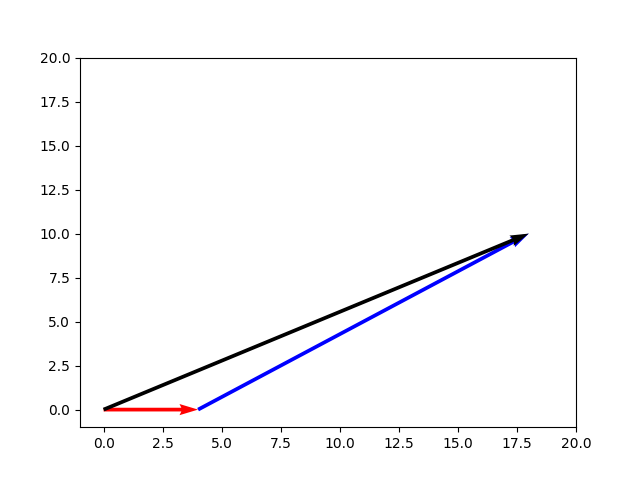
\includegraphics[scale=0.65]{3_03.png}
    \end{align*}
\end{problem}

\end{document}

